%%%%%%%%%%%%%%%%%%%%%%%%%%%%%%%%%%%%%%%%%%%%%%%%%%%%%%%%%%%%%%%%%%%%%%
% LaTeX Example: Project Report
%
% Source: http://www.howtotex.com
%
% Feel free to distribute this example, but please keep the referral
% to howtotex.com
% Date: March 2011 
% 
%%%%%%%%%%%%%%%%%%%%%%%%%%%%%%%%%%%%%%%%%%%%%%%%%%%%%%%%%%%%%%%%%%%%%%
% How to use writeLaTeX: 
%
% You edit the source code here on the left, and the preview on the
% right shows you the result within a few seconds.
%
% Bookmark this page and share the URL with your co-authors. They can
% edit at the same time!
%
% You can upload figures, bibliographies, custom classes and
% styles using the files menu.
%
% If you're new to LaTeX, the wikibook is a great place to start:
% http://en.wikibooks.org/wiki/LaTeX
%
%%%%%%%%%%%%%%%%%%%%%%%%%%%%%%%%%%%%%%%%%%%%%%%%%%%%%%%%%%%%%%%%%%%%%%
% Edit the title below to update the display in My Documents
%\title{Project Report}
%
%%% Preamble
\documentclass[paper=a4, fontsize=10pt]{scrartcl}
\usepackage[T1]{fontenc}
\usepackage{fourier}
\usepackage{caption}
\usepackage[english]{babel}							% English language/hyphenation
\usepackage[protrusion=true,expansion=true]{microtype}	
\usepackage{amsmath,amsfonts,amsthm} % Math packages
\usepackage[pdftex]{graphicx}	
\usepackage{url}
\usepackage{wrapfig}
\usepackage{multirow}


\usepackage{sidecap}
%%% Custom sectioning
\usepackage{sectsty}
\allsectionsfont{\centering \normalfont\scshape}

\usepackage{geometry}
 \geometry{
 a4paper,
 total={210mm,297mm},
 left=10mm,
 right=10mm,
 top=10mm,
 bottom=10mm,
 }
%%% Custom headers/footers (fancyhdr package)
\usepackage{fancyhdr}
\pagestyle{fancyplain}
\fancyhead{}											% No page header
\fancyfoot[L]{}											% Empty 
\fancyfoot[C]{}											% Empty
\fancyfoot[R]{\thepage}									% Pagenumbering
\renewcommand{\headrulewidth}{0pt}			% Remove header underlines
\renewcommand{\footrulewidth}{0pt}				% Remove footer underlines
\setlength{\headheight}{13.6pt}


%%% Equation and float numbering
\numberwithin{equation}{section}		% Equationnumbering: section.eq#
\numberwithin{figure}{section}			% Figurenumbering: section.fig#
\numberwithin{table}{section}				% Tablenumbering: section.tab#


%%% Maketitle metadata
\newcommand{\horrule}[1]{\rule{\linewidth}{#1}} 	% Horizontal rule

\title{
		%\vspace{-1in} 	
		\usefont{OT1}{bch}{b}{n}
		\normalfont \normalsize \textsc{University Of Bristol / LaL Orsay} \\ [25pt]
		\horrule{0.5pt} \\[0.4cm]
		\huge Assessments \\
		\horrule{2pt} \\[0.5cm]
}
\author{
		\normalfont 								\normalsize
        Renato Quagliani\\[-3pt]		\normalsize
        \today
}
\date{}


%%% Begin document
\begin{document}
\maketitle
\section{Overview of work done}
A description of the work done up to now will be described. It consists in two major blocks. The first one is related to the analysis work and it has been done from June 2014 to October 2014 , period in which i was finishing the master degree in Ferrara Unviersity and i get the NPAC master 2 at Paris Sud University. The second one is related to the work done in the context of the Upgrade of the LHCb detector consisting in the improvements of the \textit{Seeding} tracking algorithm which actually becomes the development of new algorithm , the \textit{Hybrid Seeding}.
%The analysis work regards the study of double charm $B$ decays at \textit{LHCb} while the \textit{Seeding Algorithm for the LHCb upgrade} connsists in a software development project.
\subsection{Software development Project : Seeding Algorithm for the LHCb Upgrade}
Before discuss about the work done in this domain a small introduction about the tracking and the upgrade of the \textit{LHCb} detector is mandatory.
\subsubsection{Indtroduction to LHCb and to the Upgrade Scintillating Fibre Tracker (SciFi).}
The \textit{LHCb} detector \cite{Blake1} aims to search indirect signatures of New Physics through quantum loop induced processes through the measurements of strongly suppressed Standard Model processes and studying very rare decays. In this context precision and statistics play a fundamental role. Up to now, in \textit{LHCb} and \textit{LHC}, no deviations from the Standard Model (SM) have been observed and even if \textit{LHCb} has provided the world's best measurements in some channels, it is still limited from improving them by statistics rather than systematics. Due to this the upgrade of the \textit{LHCb} forward spectrometer is mandatory in order to collect \textit{O(100)} times more data and reduce the statistics uncertainty of a factor 10 in order to be comparable with the theoretical one \cite{Blake2}\cite{Blake3}.

The \textit{LHCb} detector is designed to be a single-arm forward spectrometer aiming to the detection of particles and their decay products, and as the \textit{b} in the name of the detector suggests, it is designed to study particles containing \textit{b} and \textit{c} quarks which are produced strongly boosted in the forward and backward (lost)  directions for symmetric energies of colliding protons.\footnote{The relevant process infact is the quark-gluon fusion which can be obtained in proton proton collisions only with strongly asymmetric PDFs.}

The detailed description of the \textit{LHCb} detector can be found in \cite{Blake1}.

The data taking at \textit{LHCb} during 2011 and 2012 at LHCb are mainly determined by few steps:
\begin{itemize}
\item{Interesting events are selected by the \textit{L0 Trigger} which is implemented at the hardware level aiming to reduce the 40 \textit{MHz} bunch crossing rate to 1\textit{MHz} making use of estimation and measurements of the signature of particles having high $E_{T},p_{T}$ through the Muon stations and the calorimeter. The main reason why this is done is because the read-out system for Run-I and Run-II cannot afford an incoming rate of 40\textit{MHz}. In the upgrade infact, all the read-out will be substituted and the \textit{L0} trigger will be replaced by a software one.}
\item{\textit{High Level Trigger}: It consists in an \textit{Online} software trigger where the full reconstruction of tracks is performed. It's at this level that the tracking algorithms are run. After this step , data are stored and an \textit{Offline} reconstruction is also performed before providing usable object for data analysis. \footnote{During the Run-I, the seeding algorithm (called \textit{PatSeeding}) in the \textit{HLT} was run making use of the left-over hits coming from the \textit{Forward} algorithm. During Run-I the \textit{Seeding} was used in the online reconstruction in tandem with the \textit{Forward} as described before while in the offline reconstruction it was run as a \textit{Standalone} algorithm. For the Run-II ...to complete.}
\item{\textit{LHCb} luminosity is kept constant and it'reduced wrt other \textit{LHC} experiments of 2 orders of magnitudes. This reduction in luminosity is achieved thanks to the \textit{Luminosity Levelling} mechanism which avoid head-on collisions separating beams perpendicularly to the collision plane. This decrease of luminosity is mandatory since the main studies on \textit{b} and \textit{c} hadrons requires an extraordinary precise reconstruction of the production vertex of the $b\overline{b}$ pairs, so, the VErtex LOcator (\textit{VELO}) can be placed at very small distance from the interaction point limiting problems coming from radiation damages. \footnote{The decrease from the maximal designed luminosity of \textit{LHC} of $10^{34}cm^{-2}s^{-1}$ to the \textit{LHCb} one  $10^{32}cm^{-2}s^{-1}$ permit to reduce the average number of inelastic collisions from 27 to 0.53 and it allows to reconstruct with extraordinary precision the primary vertices.}
\end{itemize}

The track reconstruction at \textit{LHCb} is decompose in different steps. The idea is to provide different containers containing different category of tracks. The track classification at \textit{LHCb} is done depending on the path the track goes through, so it's based on the datector's hit content as shown in Fig. ~\ref{figure:Tracks}.
\begin{figure}[h]
  \begin{center}
    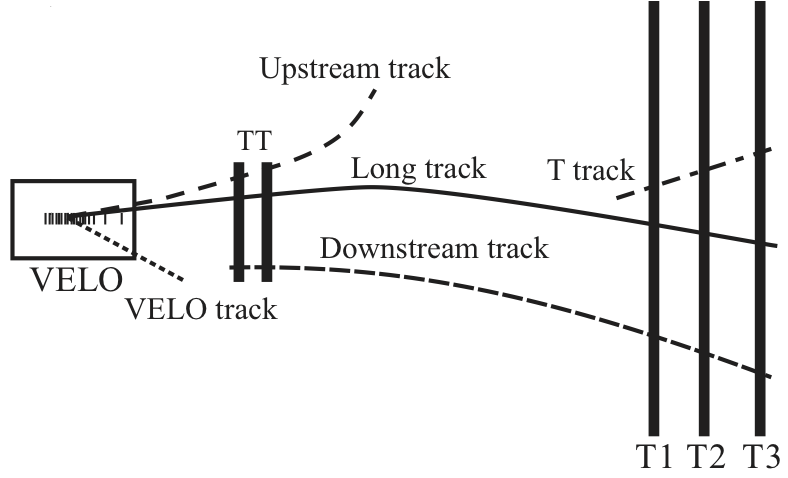
\includegraphics[width=0.5\textwidth]{Images/tracktype.png} 
  \caption{Track type at \textit{LHCb}. Velo tracks are basically straight lines since the magnetic field is almost 0 in that region. Tracks are mainly bended in the x-z\footnote{z- is the beam axis direction and the y axis is the B field line direction.} plane between the Tracker Turicensis (Upstream Tracker for the upgrade) and the T-Stations which is composed by the Inner Tracker(IT) and the Outer Tracker(OT) (Run-I and Run-II), while for the upgrade the stations will be replaced by the Scintillating Fibre tracker (SCIFI).}
  \label{figure:Tracks}
  \end{center}
\end{figure}
In the tracking system of \textit{LHCb} each track type is reconstructed by a proper algorithm and a schematic layout of how things works is given in table \ref{Table:tracks}.
\begin{table}[h]
\begin{tabular}{|l|l|l|l|l|}
\hline
Track Type & Used Detector &Algorithm(s)& Input&  Output    \\ \hline
\begin{tabular}[|l|]{@{}l@{}}Velo Tracks\\ or Velo-Segment\end{tabular} & Velo & Velo algorithm  & \multicolumn{1}{|l|}{/} & Velo         \\ \hline
\begin{tabular}[|l|]{@{}l@{}}Seed Tracks\\ or T-Tracks\end{tabular}     & \begin{tabular}[|l|]{@{}c@{}}T-Stations\\ (SciFi in upgrade)\end{tabular}                                                                                    & \multicolumn{1}{|l|}{Seeding algorithm}                                                                                             & \multicolumn{1}{|l|}{\begin{tabular}[|l|]{@{}l@{}}Allow the possible usage of\\ the leftover hits of forward.\\ If Not: Standalone Algorithm\end{tabular}} & Seed  \\ \hline
\multicolumn{1}{|l|}{\multirow{2}{*}{Long Tracks (1)}}                  & \multirow{2}{*}{\begin{tabular}[l]{@{}l@{}}Velo + TT + T-Stations\\ (TT $\rightarrow$ UT  \\ T-Stations $\rightarrow$ SciFi \\ in upgrade)\end{tabular}} & \begin{tabular}[|l|]{@{}l@{}} 1) Forward tracking:\\ Search in T-Stations knowing \\ Velo-Segment (adding also TT)\end{tabular}         & Velo Container               & \multirow{2}{*}{Long} \\ 
\multicolumn{1}{|l|}{}                                              &                                                                                                                                                            & \begin{tabular}[|l|]{@{}l@{}} 2)Matching algorithm:\\ Merge T-Tracks with Velo-Segment\\ 3)BestSelector= Forward+Matching\end{tabular} & Velo and Seed Containers                                                                                                                               &                       \\ \hline
Downstream Tracks                                                     & \multicolumn{1}{|l|}{\begin{tabular}[|l|]{@{}l@{}}T-Stations and TT\\ (SciFi and UT)\end{tabular}}                                                             & \begin{tabular}[|l|]{@{}l@{}}Downstream algorithm:\\ Use T-Tracks and\\ add TT (UT upgrade) hits\end{tabular}                         & Seed Container                                                                                                                                         & Downstream            \\ \hline Upstream Track                                                        & \multicolumn{1}{|l|}{Velo and TT} & \begin{tabular}[|l|]{@{}l@{}}Upstream algorithm:\\ Use Velo segment and \\ add TT( UT upgrade) hits\end{tabular} & Velo Container &  Upstream \\ \hline \end{tabular}
\label{Table:tracks}
\end{table}

All the tracks produced by the algorithms provided before will be reprocessed by the Kalman Filter which will reprocess the tracks assigning a sort of \textit{univoque} $\chi^{2}$ to the track and will refit them taking into account the magnetic field map and the material budget of the tracks to multiscattering correction. From a more technical point of view, each track is defined by a vector of track state $\left( x, y, t_{x}, t_{y} , \frac{q}{p} \right)_{z}^{T}$ which is then propagated by a $5X5$ matrix through the detector considering the interactions and the B-Field map. At the level of the track search done by the algorithms the main goal is to provide for each track a set of compatible hits and only at the end of the algotithm they are converted into track state.

Going back to the upgrade, a brief description on what it consists is mandatory. A small recap is given in table \ref{table:runningCondition}
\begin{table}[h]
\begin{tabular}{|l|l|l}
\hline
           & Current \textit{LHCb}          & Upgrade \textit{LHCb} \\ \hline
Luminosity & $4 \cdot 10 ^{32} cm^{-2}s^{-1}$ & $2\cdot 10^{33} cm^{-2}s^{-1}$ \\ \hline
$\mu=< \frac{Visible \quad Interactions}{Bunch Crossing}} >$ & 1.7 & 5.2 \\ \hliney
Hardware trigger & 40 \textit{MHz} to 1\textit{MHz} & 40 \textit{MHz}Full software trigger for every 25 ns bunch crossing \\
\end{tabular}
\end{table}
The reason why the \textit{L0} trigger will be removed in the upgrade is mainly because lot of analysis looking for deviations from Standard Model at \textit{LHCb} are limited by statistics and a fixed 1 \textit{MHz} readout at the upgrade running condition will be too limiting.
In order to reach the physics goals the \textit{LHCb} detector will be upgraded and the installation of the new detectors and read out is expected to happen during the long shutdown 2 in 2018/2019.

First of all the actual velo will be replaced by a lightweight hybrid pixel detector capable of 40 $MHz$ readout at the upgrade luminosity which is 5 times greater than the actual one.
Regarding the \textit{PID} detectors (\textit{RICH1 and RICH2}), the aerogel from \textit{RICH1} will be removed and the opitcal system will be modified, and , of course , new photon detectors and read-out system will be implemented. Since the \textit{L0} trigger will not be present in the upgrade, so the Scintillating Pad detector and the pre-shower which basically initiate the electromagentic and hadronic shower and applies some vetoes to the events will be removed. The calorimeters will remain the same apart of the implementation of a new read-out. The muon system also will remain the same apart of a new read out and the removal of the first station (\textit{M1}).
The trackers downstream and upstream the magnet will be insteads completely replaced. 
In particular the tracker downstream the magnet which is now made by the so-called Inner tracker \textit{IT} and the Outer Tracker\textit{OT} will be replaced by the scintillating fibre (\textit{SciFi}) detector to cope for the higher luminosity, higher occupancy and the 40 \textit{MHz} read-out.
For the current tracker system downstream the magnet two technologies are used: the Outer Tracker system is based on gaseous straw tube detector for a global resolution on the bending plane (\textit{x-z}) of around 200 $\mu m$.
The main reason why it's necessary to replace the Inner and Outer tracker is related to the Ocuupancy being too high in upgrade conditions and the fact that the electronics for them was designed for a 1MHz read-out rate. On top of that, the upgrade phase of LHCb is designed to collect an integrated luminosity of 50 $fb^{-1}$ and the detector itself is required to be resistent to the corresponding radiation damages.
The adopted solution for the upgrade is the Scintillating Fibre Tracker which is basically a tracker where the active material is actually the same of the transport one. The produced light is transported ( and shifted in wavelenght to be not absorbed by the material itself ) and collected by arrays of Silicon photomultipliers and the pitch of a single channel is designed to be equal to 250 $\mu m$.
The detector will be placed in substitution to the actual one and its design is given in \ref{Figure:Detector}.


%\begin{itemize} 
%\item Velo tracks and Velo segments : tracks are reconstructed as 3-D object and they fill the container of \textit{Velo tracks} and they are found under the assumpiton that all of them originate from the same point.
%\item \textit{T-Tracks} , i.e., tracks going through the T-Station (\textit{SciFi} for upgrade) track reconstruction, it is done by the \textit{Seeding} algorithm and it runs as a standalone algorithm (alternitavely it can run on the leftover hits of the \textit{Forward} tracking). It's mainly useful to reconstruct tracks from long-lived particles such as $K_{s}^{0}$ and $\Lambda^{0}$  and in general tracks without \textit{Velo} segment. The \textit{seeding} algorithm ouput is used then to reconstruct \textit{Downstream} tracks, as well as \textit{long} tracks.
%\item \textit{Long} tracks, which are the most interesting one for physics analysis are reconstructed mainly by two algorithms : the \textit{Forward tracking} which took as input tracks from the \textit{Velo} and propagate them into the \textit{T-station} (\textit{SciFi}) adding also additional informations from the \textit{TT} (\textit{UT} for the upgrade). The second algorithm aiming to reconstruct \textit{Long} tracks is called \textit{Matching} and it combines the output of the \textit{Velo} algorithm and the output of the \textit{Seeding} algorithm.
%\item \textit{Upstream}  tracks are reconstructed throught the \textit{Upstrem} algorithm.
%\item Long 

\subsubsection{Analysis Work : $B^{0}\rightarrow D^{0}\overline{D}^{0}K^{\ast 0}$ analysis}
Nulla consequat massa quis enim. Donec pede justo, fringilla vel, aliquet nec, vulputate eget, arcu. In enim justo, rhoncus ut, imperdiet a, venenatis vitae, justo. Nullam dictum felis eu pede mollis pretium. Integer tincidunt. Cras dapibus. Vivamus elementum semper nisi. Aenean vulputate eleifend tellus. Aenean leo ligula, porttitor eu, consequat vitae, eleifend ac, enim.

\paragraph{Heading on level 4 (paragraph)}
Lorem ipsum dolor sit amet, consectetuer adipiscing elit. Aenean commodo ligula eget dolor. Aenean massa. Cum sociis natoque penatibus et magnis dis parturient montes, nascetur ridiculus mus. Donec quam felis, ultricies nec, pellentesque eu, pretium quis, sem. Nulla consequat massa quis enim. 


\section{Choice of Thesis Topic}

\begin{itemize}
	\item First item in a list 
          \begin{itemize}
          \item First item in a list 
            \begin{itemize}
            \item First item in a list 
            \item Second item in a list 
            \end{itemize}
          \item Second item in a list 
          \end{itemize}
	\item Second item in a list 
\end{itemize}

        \begin{enumerate}
	\item First item in a list 
	\item Second item in a list 
	\item Third item in a list
        \end{enumerate}
\section{Timetable for future}
%%% End document



\begin{thebibliography}{100}
\bibitem{Blake1} LHCb Collaboration , \textit{The LHCb Detector at the LHC, JINST 3(2008) S08005}
\bibitem{Blake2} LHCb collaboration, \textit{Letter of Intent for the LHCb Upgrade}, CERN-LHCC-2011-001, March 2011.
\bibitem{Blake3} LHCb collaboration, \textit{Framework TDR for the LHCb Upgrade}, CERN-LHCC-2012-007, May 2012.
\bibitem{Blake4} LHCb collaboration, \textit{LHCb Scintillating Fibre Tracker Technical Design Report}, CERN-LHCC-2014-001; LHCb TDR 15.


\end{document}
